\documentclass[../Cours.tex]{subfiles}
\begin{document}

\chapitre{Symétries}

\partie{Symétrie axiale}

\definition{Le symétrique d'une figure $(\mathcal{F}$) par rapport à une droite $(d)$ est la figure $(\mathcal{F}')$ telle que en << repliant >> par rapport à la droite $(d)$, les figures $(\mathcal{F})$ et $(\mathcal{F}')$ se superposent.\\$(d)$ est l'axe de symétrie.}

\illustration{
\begin{center}
    \begin{tikzpicture}
        \draw (-4,-4) grid (4,2);
        \draw[line width = {0.6mm},red] (0,-4.2) -- (0,2.2);
        \node[rouge] at (0.4,-3.6) {$(d)$};
        \draw[line width = {0.6mm},vert!50!white] (-1,-4) -- (-3,-3) -- (-3,1) -- (-2,2) -- cycle;
        \draw[line width = {0.6mm},vert!50!white] (1,-4) -- (3,-3) -- (3,1) -- (2,2) -- cycle;
    \end{tikzpicture}\hspace{2cm}
    \begin{tikzpicture}
        \draw[line width = {0.6mm},red] (-1,-3) -- (1.5,3);
        \node[rouge] at (0.4,-2.6) {$(d)$};
        \draw (-2,0) -- (0,2);
        \draw[fill=noir] (-2,0) circle (0.05);
        \draw[fill=noir] (0,2) circle (0.05);
        \node[above left] at (0,2) {$B$};
        \node[left] at (-2,0) {$A$};
        \draw (-2,0) -- (0,2);
        \draw[fill=noir] (-2,0) circle (0.05);
        \draw[fill=noir] (0,2) circle (0.05);
        %\node at (0,2) {$A$};
        %\node at (0,2) {$A$};
    \end{tikzpicture}
\end{center}
}

\propriete{$A$ et $A'$ sont symétriques par rapport à $(d)$\\ $\Leftrightarrow (d)$ est la médiatrice de $[AA']$}

\propriete{\centerline{\underline{Isométrie}}
\begin{itemize}
    \item Le symétrique d'une figure est une figure de même nature.
    \item Le symétrique d'un segment est un segment de même longueur.
    \item Le symétrique d'un angle est un angle de même mesure.
\end{itemize}}

\clearpage
\partie{Symétrie centrale}

\definition{}

\begin{center}
    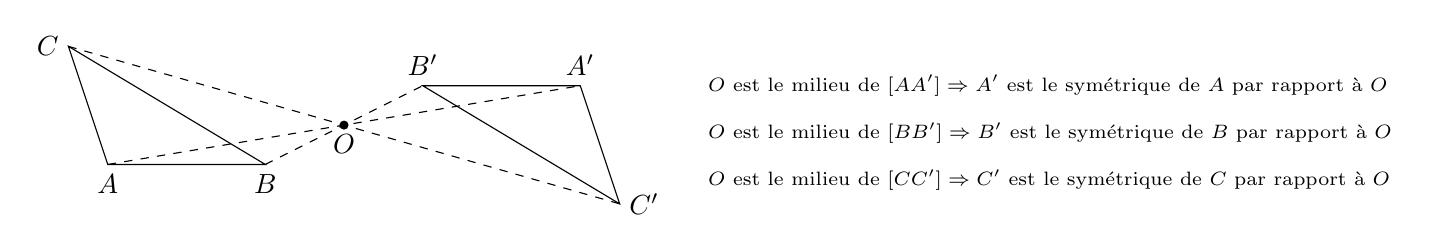
\begin{tikzpicture}
        \coordinate (A) at (0,0);
        \coordinate (B) at (2,0);
        \coordinate (C) at (-0.5,1.5);
        \coordinate (O) at (3,0.5);
        \coordinate (A') at (6,1);
        \coordinate (B') at (4,1);
        \coordinate (C') at (6.5,-0.5);
        \draw (A) node[below]{$A$} -- (B) node[below]{$B$} -- (C) node[left]{$C$} -- cycle;
        \draw[fill=black] (3,0.5) circle (0.05);
        \draw (A') node[above]{$A'$} -- (B') node[above]{$B'$} -- (C') node[right]{$C'$} -- cycle;
        \draw[dashed] (A) -- (A') (B) -- (B') (C) -- (C');
        \node[below] at (O) {$O$};
        \node[anchor=west] at (7.5,1) {\scriptsize{$O$ est le milieu de $[AA'] \Rightarrow A'$ est le symétrique de $A$ par rapport à $O$ }};
        \node[anchor=west] at (7.5,0.4) {\scriptsize{$O$ est le milieu de $[BB'] \Rightarrow B'$ est le symétrique de $B$ par rapport à $O$ }};
        \node[anchor=west] at (7.5,-0.2) {\scriptsize{$O$ est le milieu de $[CC'] \Rightarrow C'$ est le symétrique de $C$ par rapport à $O$ }};
    \end{tikzpicture}
\end{center}



\end{document}